\documentclass{thesis-ekf}

%\usepackage[T1]{fontenc}
\usepackage[english]{babel}
%\documentclass{report}
\usepackage[utf8]{inputenc}
\usepackage{graphicx} %include images
\usepackage{listings}
\usepackage{minted} %write code snippets
\usepackage{tcolorbox} % border shade for inline code
\usepackage{amsmath,amsfonts}
\usepackage{titlesec} % make arbitrary amound of nested header with numbers
\usepackage{enumitem}
\usepackage{url}
\usepackage[style=authortitle,backend=bibtex]{biblatex}
\DeclareFieldFormat[article,book,inbook,incollection,inproceedings,patent,thesis,unpublished]{title}{#1}

\addbibresource{bibliography.bib}
\usepackage{hyperref}



% for nested enumration
\setlist[enumerate,1]{label=\arabic*}
\setlist[enumerate,2]{label=\theenumi.\arabic*}
%\setlist[enumerate,3]{label=\theenumii.\arabic*}
\setcounter{secnumdepth}{6}


\graphicspath{ {./usedImages/} }

% !TeX TXS-program:compile = txs:///pdflatex/[--shell-escape]

\setminted[python]{breaklines, framesep=2mm, fontsize=\footnotesize, numbersep=5pt, xleftmargin=20pt,linenos}
\setminted[text]{breaklines, framesep=2mm, fontsize=\footnotesize, numbersep=5pt, xleftmargin=20pt,linenos}

\hypersetup{
	colorlinks=true,
	linkcolor=blue,
	filecolor=magenta,      
	urlcolor=cyan,
	pdfpagemode=FullScreen,
}


\newtcbox{\myovalbox}{on line,colback=lightgray,boxrule=0pt,arc=2pt, boxsep=2pt, left=0pt, right=0pt, top=0pt, bottom=0pt}
\newcommand{\inlineCode}[1]{{\myovalbox{#1}}} % Highlight text that has been added




\begin{document}
	
	\author{Ahmed Mohamed M. Mahfouz Gadalla}
	\title{AI beats a game}
	\institute{Institute of Mathematics and Informatics}
	\supervisor{Dr. Kovásznai Gergely}
	\city{Eger}
	\date{April 2023}
	
	
	\maketitle
	\tableofcontents
	
	\chapter*{Dedication}
This journey of three years is coming to an end, but it didn't come to this point in the period of only these years. It is the sum of my life up until this point. This is why I want to thank, by far, my parents, \textbf{Amal Hady} and \textbf{Mohamed Mahfouz}. Always putting my priorities before theirs, being the important part of me, and making me the person I am today. Thanking my mom for taking care of me with all the characteristics (good and bad) in myself.  The idea of having an AI that beats the game is inspired from my dad winning over me when I was a child in racing games. I decided to make a game where I wouldn't have to touch the controller to get a higher score than him. From my heart, I thank both of you.
	
Now that the emotional part is over. There are people who shaped the programmer inside of me today, to the point where he is capable of developing the thesis that is in front of you, my classmates, and my supervisor, \textbf{Dr. Kovásznai Gergely}. His work with me through the studying period, sending emails for him back and forth, really can make it up to him. Not only by guiding me, but also by giving me the steps of what to do. 



	\chapter{Introduction}





	\chapter{Related work}

"God is the one who endowed man with reason, and the mind is the basis of everything. The mind is light and knowledge is a result, and so every knowledge is light" -Jābir ibn Hayyān. This work wasn’t totally completed in one day, and wasn’t completed from beginning to end without the help of online sources. Some of them are in the form of videos, and others are in the form of papers. Most of the sources that will be found here, are more related to the game field to make the graphics of the game and the logic for the player. While the papers have taken the shape of an implemented (Python) library to be used.

On the other hand, the related sources to the field of AI, are implemented as (Python) library to be used. It can be found in papers that require more than average knowledge about basic concepts in this field. I tried to clear most of them in the \hyperref[sec:101-ai]{101 AI} part.

The algorithm itself have been used in other low-budget games with the same purpose of making the environment more interactive, like:

\begin{itemize}
\item Galactic Arms Race (GAR): The game is about a galactic war and there are weapons included as part of the game. "In GAR, all player weapons are generated by the (content-generating NEAT) cgNEAT algorithm based on weapon usage statistics. However, cgNEAT does not simply respawn weapons that people like. Rather, it creates new weapons that elaborate on the ones that have been popular in the past" \href{http://galacticarmsrace.blogspot.com/p/research.html}{Galactic Arms Race: Research}.

\item Dance Evolution: is interactive application made by the researcher behind the N.E.A.T algorithm "Kenneth O. Stanley". The game allows you to choose a song, and then a set of dancers will dance to it. When you choose a dancer, it will be the base for others to follow.

\end{itemize}

So as an implementation in the field of games by the creator, there hasn't been a single one that was made recently (in the last 10 years). While there have been little implementation to the idea of having N.E.A.T algorithm to play a game. One is either developed from ground to up like this tutorial \href{https://www.youtube.com/watch?v=2f6TmKm7yx0&t}{Python Pong AI Tutorial - Using NEAT (by Tim Rescica)}.  Others have made it on an open source game from another library and add their own tweaks to the library to fit the game, like \href{https://www.youtube.com/watch?v=5RR1T_-zVws&t}{A.I. Learns to Play Sonic the Hedgehog - NEAT Explained! (by Forrest Knight)} where he takes Sonic the Hedgehog module from Gymnasium (formally known as GymAI by openAI) and implement the N.E.A.T algorithm on it.

My implementation will be different from all of the previous examples because:
\begin{enumerate}
\item All the components in the game are pixel-generated, means that there isn't a single image used in the whole game.
\item A full in-depth explanation of the AI is discussed here. As this is the first AI project for me, I elaborate on the details here as if it were my first time learning it. The methodology used in the questions part is the Feynman Technique.
\end{enumerate}




	
	\chapter{Technologies}

The project itself was purely an idea I got as an application for AI. There would still be a need for sources to help me get turn idea into something real that is applicable. The problem I had mostly with the implementation was getting the documentation of PyGame and knowing what the best implementation was for each function I wanted to implement. While making an a game for PC, you have to think wisely about the sources and how to use them in your favour.

\section{ Running library (PyGame)}
The base for the game is made on \href{(https://www.pygame.org/wiki/about}{PyGame} library. It is "a set of Python modules designed for writing video games. PyGame allows you to create fully featured games and multimedia programs in the Python language". You can also control anything in the game itself, as you would have a main loop that you can think about as the frames per second of the game. Getting to know the library was easy, because of my past experience with Python, and the documentation was easy. The library has been around for some time now, which made it easy to get a 101 guide on how to get the basics.



There was one main part while making the game, developing the GUI. Making the interface for the game was a little hard as it would take much time to learn the drawing functions, such as writing a text on the screen. During the AI training, there is information that shows on the screen to make reading the log easy, like the \textbf{score} and \textbf{generation number} along side with the \textbf{genome ID}. Writing the info isn’t as easy as dragging and dropping like most gaming engines, but everything has to be coded on the screen with x and y coordinates.
\begin{figure}[H]
	\centering
	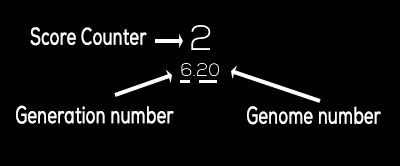
\includegraphics[width=0.7\linewidth]{usedImages/scoreFrame}
	\caption{illustration for info on the score side	}
	\label{fig:scoreframe}
\end{figure}

What is good about the PyGame library is that it allows me to have dynamic game dimensions. The screen resolution for the game while developing it was $400*800$, but as most of the components on the screen are made in relation to the screen resolution the user define from the code, then you wouldn't have to change every component location from the code, the game will already do it by itself.

\section{AI library (N.E.A.T Algorithm)}\label{sec:ai-library-neat-algorithm}
"\textbf{N}euro \textbf{E}volution of \textbf{A}ugmented \textbf{T}opologies. And this is what's known as a genetic algorithm" \href{https://www.youtube.com/watch?v=2f6TmKm7yx0}{[Python Pong AI Tutorial - Using NEAT - YouTube}. Think of it as the way that is used in humans to learn (refer to the example of the \hyperref[sec:ai-life-example]{kid and the ball} in further reading) and the natural selection of the ones that perform well as humans and are smarter, they managed to reproduce until today. Unlike the others, who were not fortunate enough to have what it takes to survive in different scenarios.

In other words, to explain it "There is a larger category called TWEANN stands for \textbf{T}opology and \textbf{W}eight \textbf{E}volving \textbf{A}rtificial \textbf{N}eural \textbf{N}etworks" \href{https://www.youtube.com/watch?v=5RR1T_-zVws&}{A.I. Learns to Play Sonic the Hedgehog - NEAT Explained! - YouTube}" These are algorithms that not only evolve the strength of the connection weight for a fixed network topology but actually evolves both the topology of the network and its weights." The scientists behind the neat algorithm identified three major challenges for tweanns:

\begin{enumerate} \label{list:3tweanns}
	\item Meaningful crossover: by tracking genes through historical markings.\\
This stops the algorithm from blindly crossing over the genomes of two neural networks and creating unnormally mutated neural networks. There are two ways to progress through a user-specified number of generations, "with each generation being produced by reproduction (either sexual or asexual) and mutation of the most fit individuals of the previous generation" \href{https://neat-python.readthedocs.io/en/latest/neat_overview.html}{NEAT Overview}.
	\begin{itemize}
		\item Sexual: means that the new generation will be made out of the best-performing genomes from \textbf{the previous generation}.
		\item Asexual: algorithm will \textbf{generate a random genome} to reproduce with the genomes with the highest fitness score to make the new generation.
	\end{itemize}
	
	\item Speciation: protecting structural innervation through speciation.\\
	That protects new structures, as they are typically low on hidden network numbers, allowing them to optimize with each other on their own. You can say category before we eliminate them. This is done by splitting up the population into several species based on the similarity of topology, connections between neurons, and their weights and biases. They only compete within their species because some of them who aren’t performing well at present, can perform well in the future after the right mutation with each other without the need to eliminate them now.
	\item Structure complexity: incrementally growing from minimal structure.\\
It prevents the algorithm from creating complex networks at the beginning of the new generation that may have to later reduce the number of nodes and connections. They did this by starting all networks with no hidden layers between the input and output layers. NN only has a series of connection genes between them, and if it is found to be useful and necessary to tweak the output a little, then it can involve complexity.
\end{enumerate}

They designed N.E.A.T to specifically address each one of the above characteristics. Point (2) and (3) will be explained more in details at the \hyperref[sec:explain-the-log]{explain the log} from timeline chapter.




	
	
The first step of developing the game was choosing a programming language that would be helpful in both showing graphics on screen and implement an AI algorithm. The only option that was convenient enough was python as:

\begin{enumerate}
	\item The most famous programming language with AI libraries that have a good documentation.
	\item It is OOP, which means I can have a class for each component of the game easily to make an instance for the AI to train from.
	\item A library to draw graphic on screen while it won't need heavy CPU usage that won't throttle the process of AI learning 
\end{enumerate}

Choosing a library for the game was the first step as it would define the characteristics. I went for \textbf{PyGame} because it was nearly the only one that is good enough with documentation to start with, and quit enough, the main focus isn't about making a game that will have that much of physics in it and 3d animation. For now, the imagined picture of the game is a rectangle as a screen that will have two main component of the game, a wave that is on one side of the screen vertically and one on the other side with the only difference is 350px (the starting amplitude is 50px and the screen width is 400px) and a ball that the \textbf{only purpose for it is to survive as much as it can, without hitting any of the sides of the wave}.\\


I'm minimalist when it comes to developing things, like there wouldn't be splash screen all over, and hard controls, not even hard rules, and it will be the approach I'm following with the game, to break it into steps:

\begin{enumerate}
	\item The accent colour of the game will be black as a background
	\item White will be used to show elements 
	\item Score counter on top
	  \begin{enumerate}
		\item AI mode: show generation and genome number
		\item AI mode: show total runtime
		\item AI mode: show the vision of the ball
	\end{enumerate}
\end{enumerate}

During the writing here, I will raise some questions that might come to your mind while working on some parts (as they might have came to me too) and will try to answer them at the end of every section in the chapter.

\section{Develop the game}\label{develop-the-game}

The files layout of the game will be an \inlineCode{AI.py} file in the root folder, then subfolder named \inlineCode{SurviveLine} with 3 files in it \inlineCode{ballFunc.py}, \inlineCode{waveFunc.py} and \inlineCode{game.py}. To make it easy to make instance of the game, will create a file named \inlineCode{\_\_init\_\_.py} that will only have one line it it \inlineCode{from .game import Game} that means we will have a \inlineCode{Class Game():} in the \inlineCode{game.py} and it is used to call the \inlineCode{game} function as a library in the \inlineCode{AI.py} file (as it is in another folder) and make instance from it. Every major component will have its own class in file to refer later. 

\subsection{Wave functionality}\label{wave-functionality}
To get the base function of wave, there would be a lot of functions to cover like:

\begin{minted}{python}
def draw(self, Display):
	#increase the FPS of game
def changeSpeed(self):
	#change the wave aplitude and increase the wave gap
def changeWave(self):
	#generate a new point on Y axis
def generateWave(self):
	#add point to the list of points
def addPoint(self, index, point):
	#check if there is a gap 
def checkGap(self):
	#function to fill it
def fillGap(self, gap, gapDirection):
	#reset all the self. variable that are made in __init__ class 
def reset(self):
\end{minted}

most of them are self explanatory, but the ones that need more dive into details are the \inlineCode{generateWave}, \inlineCode{checkGap} and \inlineCode{fillGap}.

\subsubsection{Generate wave}


The starting point of the game, in the \inlineCode{waveFunc.py} to make a main class \inlineCode{Class Wave():} with an equation that can generate a wave and at the same time I can change in the variables of the wave to make it harder for the player. These variable are wave amplitude\footnote{is the maximum or lowest height the wave can go in one point to up or down.} or wave frequency\footnote{a number of waves that can go through a fixed distance in amount of time.}.

With all of this in calculation which means that I can make the game harder by making the behaviour unexpected for the next move, also to go extra step, there will be a decrease in the gap between the two waves to limit the player's movement.

\begin{minted}{python}
pointsList_XCord = int((self.HDisplay/2) + self.WaveAmplitude* math.sin(self.waveFreq * ((float(0)/-self.WDisplay)*(2*math.pi) + (time.time()))))
\end{minted}
as you can see, there are some variables that have the \inlineCode{self.} before, that are defined as:

\begin{listing}[!ht]
\begin{minted}{python}
	def __init__(self, wDisplay, hDisplay):
		self.WDisplay = wDisplay
		self.HDisplay = hDisplay
		self.ScoreCount = 0  
		self.waveFreq = 1  # changes difficulty part
		self.WaveGap = 0
		self.GameSpeed = 2  # to increment the difference in time to speed the FPS
		self.FPS = 60
		self.WaveAmplitude = 50
		self.PointsI = 0  # index to loop inside the points list
		self.PointsList = [0]*800
\end{minted}
\caption{the self variable in waveFunc file.}
\label{code:waveFunc self}
\end{listing}


These are the variables that are only (and not specifically) linked to the wave functions, and this is where an important functionality of OOP comes in. Encapsulation is the OOP functionality which means to get all the related data to a class (which is wave class at this point), if it is needed in other classes, then an instance of class wave can be made then the new variable can be used from it.

The equation in figure \ref{code:waveFunc self}  is going to store the X axis coordinates in a list called \inlineCode{PointsList} for the sake of adding points to it once they are generated and show them on screen one by one as if it is loading, because if there isn't a list, then the wave would be a steady visual sine wave (without changing amplitude or frequency yet), this part of code is placed in \inlineCode{def generateWave(self)} function.

There have to be more condition to make the points be generated without disorder, like one point won't be in the other half of screen, which means that when the 350px is added to it, it will be out of the borders of the display.


\subsubsection{Check gap}
After generating a point, with the change in amplitude, the next point that is added to list of points doesn't have a difference of only 1px with the one before it, so it means that there will be a different line segments in the list and a gap between the old point and the new one. To overcome this, after a point is generated, there is a \inlineCode{for loop} that checks if there is only one pixel gap between it (the new point) and the point before it, either it is minus or negative as the gap can be to left or right side.

\begin{figure}[H]
	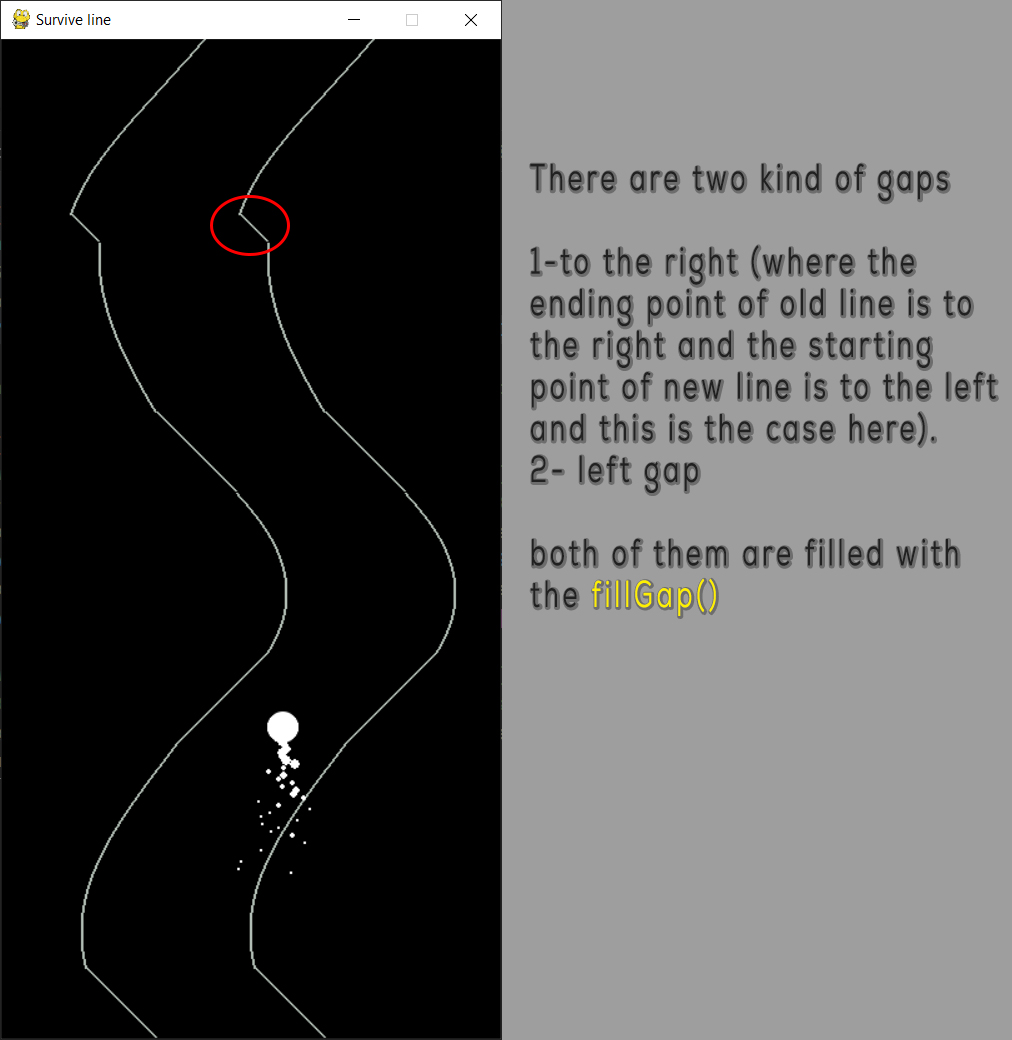
\includegraphics[scale=0.5]{filledGap}
\end{figure}

\subsubsection{Fill gap}
If there is one part which took the most in developing, I would say it is this part, because there were different approaches to solve the problem. First one is either to move the point on y-axis by the gap then make a straight line from the old line segment to it, and the second one was to get the point just to be minus on the x-axis then be linked to it. The first option was better for the sake of visibility and not effecting the next point respectively. There were lots of ways (or you can say conditions) that needs to be covered in the point list, for example what if the gap is at the end of list?  will throw "out of index error" when trying to shift the new point by the amount of gap. One way to cover this is by removing amount of points from the start of the list, then add the same amount at the end where you need it.

Say that the gap is over the limit of list (800Px), dealing with it before was just to make the gap limited to the end of list, so if the point is at index 797 and the gap is 10 (that means there will be an "out of index" error at extra index 6) so it was just to make it limited to  \inlineCode{gap = DISPLAY\_H - POINTS\_I - 1} but the problem is that it wouldn't work on high scale when the amplitude gets higher.
To deal with it is to remove the over-points in gap from the beginning of the list and add empty points of the same amount at the end then make the index go back to the new index, (back to the same example). It will remove 6 points from the beginning of list then add empty 6 points to the end, and shift the index to 6 points in the back so it stays with the new point.

\begin{listing}[H]
\begin{minted}{python}
if self.PointsI + (gap) >= self.HDisplay-1:
	untilEnd = self.HDisplay-self.PointsI
	toAddFromStart = abs(gap-untilEnd)
	del self.PointsList[:toAddFromStart]
	toAdd = [0]*toAddFromStart
	self.PointsList.extend(toAdd)
	self.PointsI -= toAddFromStart
	gap -= 1
\end{minted}
\end{listing}

with every line here looking weirdly by itself, you would need some explanation:

\begin{itemize}
	\item Line 2: calculates the difference between the ending point of list and the starting point of gap.
	\item Line 3: get the difference in gap and the point.
	\item Line 4: delete the amount of point from the beginning of list.
	\item Line 5: create empty list with the amount of delete points from beginning of list.
\end{itemize}

Now with the condition being fulfilled, it comes to fill the gap itself. There would be two options, if the gap is negative or positive, but I will discuss the negative gap and the other one have the same implementation with the difference being the sign.

\begin{listing}[H]
	\begin{minted}{python}
if (gapDirection):
# to move the point according to gap
	self.PointsList[self.PointsI + gap] = self.PointsList[self.PointsI]
	self.PointsList[self.PointsI] = 0
	#the step is different for gap direction, as it would be -1 or +1
	for x in range(self.PointsList[self.PointsI-1], self.PointsList[self.PointsI+gap]-1, (gap//gap)):
		self.PointsList[insideY] = x+1
		if insideY < 799:
			insideY += 1
	\end{minted}
\end{listing}

First it moves the first point in the new line segment by the amount of gap, then resets the old value of it to zero (as it will be part in the straight line). Secondly is a for loop to fill the points incrementally starting from the last point in the old line segment to the new point.

\subsubsection{ Second way to fill the gap}

Fill the gap was basically working on the base of shifting the point on Y-axis, but there might be another approach to tackle this ( the second way I talked about in fixing the problem of gap).

Thinking that it will take more effort to move the point in new line segment in the position that corresponds to the gap, then make a line between the old line segment and the new one. That is a lot to think about, there can be a different way. What if we change the point on x-axis? just to make it close to the old one, I know it is a bit of cheating, but as long as it works, then it is good.

The idea is that, if I can calculate the gap (which I already know) then decrease the new point by the amount of gap + 1 (if it is a positive gap) and will be -1 if it is a negative gap, you may ask, "why didn't you use absolute value for amount of gap as left is the same as right?" because then this would mean that the wave would increment in one way which depends if it is +1 or -1.

The newly implemented function is called \inlineCode{def shiftOnXAxis(self, newPoint)} in \inlineCode{waveFunc.py}.


\subsection{Ball functionality}\label{ball-functionality}
The main focus when working on the ball was to make it as simple as it can be, so a new instance can be done from it without the need to store a self-genome variable, and every genome would have its own variables that can be changed with a new instance made.

\subsubsection{Draw ball}\label{draw-ball}
As the game is based on a \textbf{ball} that survives a line, then I need to display a ball and not a circle (google the difference). There isn't a function to draw a filled ball in one line, so I have to draw an empty circle then fill it. The function \inlineCode{pygame.gfxdraw.aacircle} will draw an anti-aliased circle and \inlineCode{pygame.gfxdraw.filled{\_}circle} draw a filled circle inside of it, then draw a fake rectangle around them with \inlineCode{pygame.Rect} that will deal with the collision (will discuss it in the display game section).

\subsubsection{Generate particles}\label{generate-particles}
This part is little on logic than the other because it was made for the visuality of the game, no output coming out of it to make the game faster or improve something, but it would add a little bit of a characteristic to the game and the vision I have for it.

The particles are made to be in the position of the ball and generate as a way to look like a combustion engine steam coming out ot it, so there are three things to notice here.
\begin{itemize}
\item Location: where the particles will start and their ending point.
\item Velocity: the amount of particles that will be generated in a second.
\item Time: how long they will last on the screen.
\end{itemize}

With this in consideration, we can start writing a function for it 

\begin{listing}[H]
	\begin{minted}{python}
def generateParticles(self):
	Loc =[self.ballCordX, self.ballCordY] 
	Vel = [random.randint(0, 20) / 10 - 1, -3]
	Timer = random.randint(4, 6)
	self.Particles.append([Loc, Vel, Timer])
	for particle in self.Particles:
		particle[0][0] -= particle[1][0]
		particle[0][1] -= particle[1][1]
		particle[2] -= 0.1
		
		pygame.draw.circle(self.GameDisplay, (255, 255, 255), [int(particle[0][0]), int(particle[0][1])], int(particle[2]))
		if particle[2] <= 0:
			self.Particles.remove(particle)
	\end{minted}
\end{listing}

In the \inlineCode{Vel} variable deceleration part, it makes sure that the value we would get, would be a random number between {-1, 1}. The \inlineCode{Timer} to give chaos to the particles so not all of them are released at the same time.

The code would add to the list of particles a new particle with these random starting values, then the \inlineCode{for loop} process each value on its own.

\begin{itemize}
\item Line 7: it process the position on X-axis to the velocity also on the X-axis, same would happen to the Y-coordinates.
\item \inlineCode{particles[2]} is to reduce the particle radius by 0.1 in every frame (which is every loop then).
\item If condition at the end to remove the particle from the list so it wouldn't take much of space with more runtime.
\end{itemize}

This function is possible thanks to [Particles - Pygame Tutorial - YouTube](https://www.youtube.com/watch?v=F69-t33e8tk)

\section{Display the game}\label{display-the-game}




\section{Create AI}\label{create-ai}

\subsection{101 AI}\label{101-ai}


\subsection{What is N.E.A.T?}\label{what-is-neat}

 
\subsection{Tweak AI}\label{tweak-ai}

\subsection{Observation}\label{Observation}

\subsection{Explain the log}\label{explain-the-log]}
 
 
 
 
 
 
 
 
 
 
 


	\chapter{Testing}
At first time running the algorithm, the input vision for the ball to the wave was from the centre of the ball to both sides of the wave as a single point. That made it hard for the ball to find its way (or have a futuristic vision, as you can say). There would be a change in the wave curve and the ball could not detect it, so the idea came of having more range for the ball to see. It would calculate the distance between the ball rectangle and the left or right side of the wave in more than one point.

To get more into it with numbers, there would be a notice of the ball having a weird sense of getting to know its "new" sense of wider vision diameter. The ball would take about 20 generations just to start moving more randomly left and right. This is made when the ball had only the vision of its 24-pixel diameter (12 px as radius) and then the extra step of plus 50 pixels, getting this info in a nutshell:
\begin{itemize}
	\item \textbf{One point vision}: good as start and better CPU wise.
	\item \textbf{Diameter vision +20}: best one in score yet (117 points in generation 89).
	\item \textbf{Diameter +50 points}: No learning even after nearly 300 generations.
\end{itemize}

The reason to increase the vision for the ball (even though it was working fine) is that I wanted to test how long it would take for the ball to get used to the new (increased) amount of lines. I can tell you that it took long enough.

\begin{figure}[H]
	\centering
	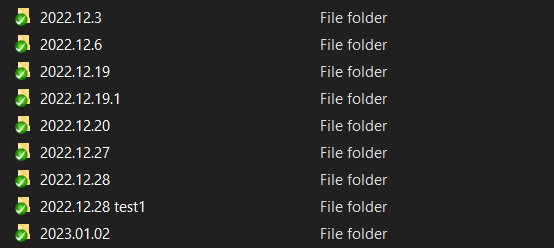
\includegraphics[width=0.7\linewidth]{usedImages/numTrainingSessions}
	\caption{A couple of training sessions}
	\label{fig:numtrainingsessions}
\end{figure}


At this point in the game, I implemented the increased speed of wave *4 that improved the learning speed. With normal fps, it would take 8 hours and 15 minutes for 37 generations, but the new one (with a limitation of 4 times the speed, not more) takes 5 hours and 15 minutes for 100 generations to work. That is four times the normal running time of a normal pace of game for a human to play it.

When I increased the vision lines and set the generation threshold to be 300 generations instead of 100 (as in \hyperref[sec:count-distance]{Count Distance} section). Let the laptop run as much as it needs. It took more than 15 hours to finish 294 generations and 11 genomes, when I went back to check the log, none of them managed to pass the 3000 fitness score. That means that none of them had a good intuition about the lines to move left or right and at least overcome one curve in the wave. From this, the amount of vision numbers increased = more time in training.

There is a small box that is shown around the ball, it is called ballRect and is mentioned a lot in the \hyperref[sec:count-distance]{Count Distance} and \hyperref[sec:collision]{Collision}. ballRect is shown to check if the genome did terminate for an actual collision or because it reached the threshold, like the case here in this video.

In order to save as much CPU power as possible during the learning process, the box is shown only when fitness is over 50. In addition to some extra visuals in the game, such as the particles behind the ball, all of them can be viewed again with a key for each one:
\begin{itemize}
	\item \inlineCode{v Key} to shown \textbf{v}ision
	\item \inlineCode{b key} to show the \textbf{b}allRect
	\item \inlineCode{p key} to show the \textbf{p}articles
\end{itemize}
	
	\chapter{Summary}
Here, I will review the findings from the previous sections. I will consider the implications of AI in this paper regarding its performance compared to a human playing a game. I will also include a discussion of any lessons learned from the project and any future work that can be done.

\section{The game development}
The progress of the game took most of the time due to the lack of sources in the PyGame library with the right functions that I was looking for then. Generating the function was the part that took most of the time. I remember that I spent more than a month trying to figure out a way to make the wave have a random amplitude so the player wouldn't cheat in the game. The problem was finding a way to make the wave one sequence after generating with the new amplitude, as it would shift the new sequence by a specific amount of pixels on the x-axis, either positively or negatively, in relation to the last point in the old sequence.
\begin{figure}[H]
	\centering
	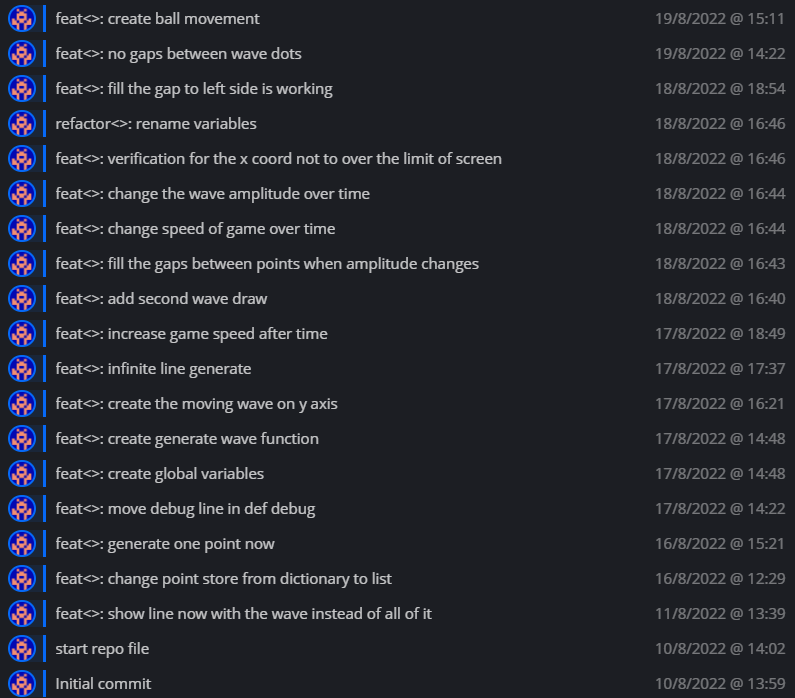
\includegraphics[width=0.7\linewidth]{usedImages/repoStart}
	\caption[]{the start of game repository on GitHub}
	\label{fig:repostart}
\end{figure}

Dealing with the other parts, such as, making the game follow the principle of encapsulation, took more than 3 days of continued work. Something I had before was the problem of having one file that did the functionality for all components of the game. For instance, the reset function that existed in ball functions is responsible for resetting the whole game, including wave-related variables. It is preferable to create a class for the wave and then include a function in it to reset the associated variables. You can call the wave functions whenever you want.

In my opinion, this is preferable, because I would be confused about which variables to call and would benefit from a better file management for each component of the game.
\begin{figure}[H]
	\centering
	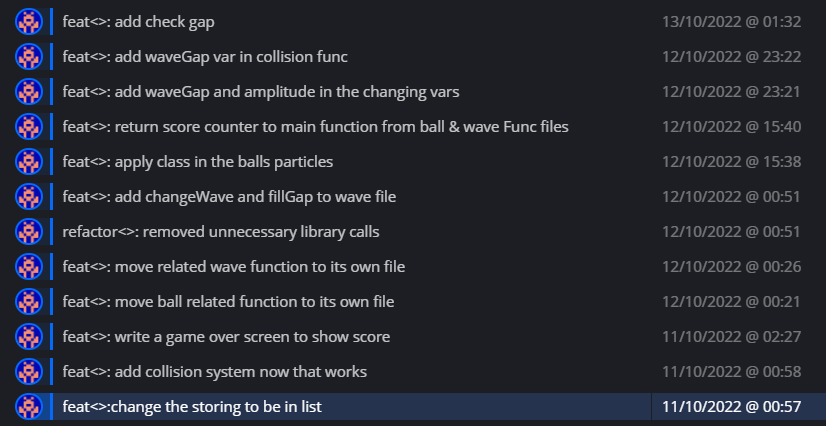
\includegraphics[width=0.7\linewidth]{usedImages/repoEncapsulation}
	\caption[]{Time it took to implement the new layout in encapsulation}
	\label{fig:repoencapsulation}
\end{figure}

The repository can be accessed from this link \citetitle{Mahfouz_Survive_Line_2023}. The game, along with running footage, can be viewed on my website \citetitle{Survive_Line_-_Ahmed_Mahfouz} for more visuality and the learning curve about it.

\section{The AI tweaking}

This part didn't require much tweaking, as it was just to leave the laptop to do the training sessions for the night and check the log in the morning. To compare between each generation, I had to add extra \inlineCode{print()} sentences in the log to keep track of them. It was also important to record the sessions with OBS, as I could navigate easily from the output code to the part in the video and then tweak it as much as I could for the next generation.


	\printbibliography

	
\end{document}